\documentclass[12pt, a4paper]{article}
\usepackage[utf8]{inputenc}
\usepackage{graphicx}    % Inserting images
\usepackage{amsmath}     % Mathematical formulas
\usepackage{algorithm}   % Pseudocode for algorithms
\usepackage{algpseudocode}
\usepackage{hyperref}    % Hyperlinks
\usepackage{natbib}      % Reference management
\usepackage[UTF8]{ctex}  % Loading Chinese support package
\usepackage{xeCJK}       % More flexible Chinese support
\usepackage{geometry}    % Setting page margins
\usepackage{eso-pic}     % Adding background images to pages

\geometry{
    margin=0cm,  % Setting margins to 0 to ensure images occupy the entire page
    paper=a4paper
}

% Using eso-pic package to add background images
\AddToShipoutPictureBG{%
    \put(0,0){
\includegraphics[width=\paperwidth, height=\paperheight, keepaspectratio]{cover.jpg}}%
}

\title{From Trojan Horses to Meme Warfare —— Sovereign Battles in the Bit Torrent}
\author{Weiyichang Zou\\ZZU\\2480237998@qq.com}
\date{April 26, 2025}

\begin{document}

\thispagestyle{empty}  % Remove page number
\null
\newpage
% Clear background image settings
\ClearShipoutPictureBG
\AddToShipoutPictureBG{%
    \put(0,0){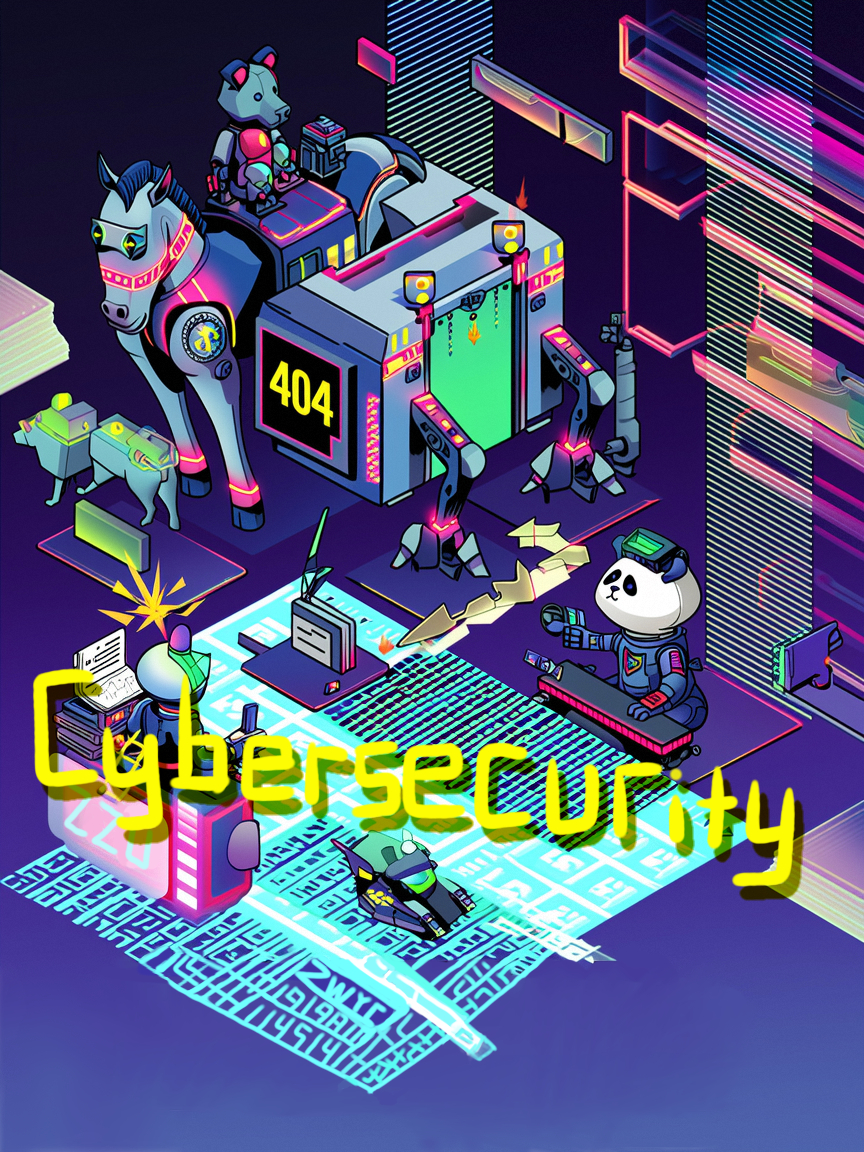
\includegraphics[width=\paperwidth, height=\paperheight, keepaspectratio]{cover2.jpg}}%
}
\thispagestyle{empty}  % Remove page number
\null
\newpage
% Clear background image settings
\ClearShipoutPictureBG

\newgeometry{margin=1in}

\maketitle

% Abstract
\renewcommand{\abstractname}{Abstract}
\begin{abstract}\

With the rapid development of information technology, cyberspace has emerged as a critical battlefield in modern national defense. Cybersecurity and information security technologies play a crucial role in safeguarding national security, ensuring the integrity of military communication and command systems, and advancing the informatization of national defense. This paper analyzes the impact of cyber warfare on national defense security by examining case studies of cyberattacks during the Ukraine conflict. It further explores the evolving trends of information security technologies in future warfare, while investigating their specific applications in defense domains such as military communication, command systems, intelligence systems, and the integration of artificial intelligence technologies. Finally, the paper discusses the roles and responsibilities of students specializing in information security in the context of defense informatization, providing both theoretical insights and practical guidance for modern national defense development.


\textbf{Key Words:} Cybersecurity, Information Security Technology, Cyber Warfare, National Defense Security, Ukraine Conflict, Military Communication, Command Systems, Artificial Intelligence, National Defense Informatization, Information Security Education, Future Warfare Trends, Cybersecurity Offense and Defense, Defense Informatization Development
\end{abstract}

\newpage

% Table of Contents
\renewcommand{\contentsname}{Contents}

\tableofcontents

% Main Body
\section{Introduction}\label{sec:introduction}
\subsection{Research Background}

\textbf{There can be no national security without cyber security, no stable functioning of the economy and society, and no reliable safeguarding of the interests of the broad masses of the people.}  

\textit{—President Xi Jinping, \textbf{Address at the National Cybersecurity and Informatization Work Conference}, April 20, 2018.}\citep{ref0}

To clarify China's major positions on cyberspace development and security, guide China's cybersecurity efforts, and safeguard national sovereignty, security, and development interests in cyberspace, the National Internet Information Office formulated the \textit{National Cybersecurity Strategy} with the approval of the Central Cybersecurity and Informatization Leading Group. \citep{ref1}\citep{ref2}\cite{ref3}\cite{ref4}\cite{ref5}\cite{ref6}\cite{ref7}\cite{ref8}

\subsection{Research Motivation}
As the global process of informatization accelerates, cyberspace has become a critical domain of competition among nations. The concealment, efficiency, and traceability challenges of cyberattacks make them indispensable tools in modern warfare, thus warranting in-depth study.

\subsection{Research Objectives}
The objectives of this paper are:
\begin{itemize}
    \item To explore the importance of cyberspace security in modern national defense, analyze its definition, current status, and strategic position in national security.
    \item To examine the impact of cyber warfare on national defense security through case studies, analyzing the profound effects of cyberattacks on the course of war, social order, and national decision-making.
    \item To investigate the role of information security technologies in modern warfare, analyzing how they influence the outcomes of war, including operational efficiency, intelligence, and psychological warfare.
    \item To study the development trends of information security technologies in future warfare, exploring the application prospects of emerging technologies such as artificial intelligence and quantum encryption in the field of information security.
    \item To discuss the roles and responsibilities of students specializing in information security in the context of defense informatization.
\end{itemize}

\subsection{Main Contributions}
Innovations:
\begin{itemize}
    \item A macro-level analysis of the importance of cyberspace security in national defense.
    \item A case-study analysis of the impact of cyberspace security on the course of war.
    \item An analysis of the role of information security technologies in warfare.
    \item An exploration of the development trends of information security technologies in future warfare.
    \item A discussion of the roles and responsibilities of information security students in defense informatization.
\end{itemize}

% Related Work
\section{Related Work}\label{sec:related-work}
Previous research has provided in-depth insights into the relationship between cyberspace security and national security. However, these studies are either insufficiently detailed or outdated.

This paper adopts a data collection and analysis approach, combining real-world case studies to conduct an in-depth investigation into the relationship between cyberspace security and national security.

Unlike previous studies, this paper adopts a more macro perspective and employs a formula-based methodology.

\section{The Importance of Cyberspace Security in Modern National Defense}\label{sec:importance}

\subsection{Definition of Cyberspace Security}
Cybersecurity (also known as computer security, digital security, or information technology (IT) security) is a subdiscipline within the field of information security. It involves the protection of computer software, systems, and networks from threats that could lead to unauthorized information disclosure, theft, or damage to hardware, software, or data, as well as disruptions or misdirections of the services they provide. \citep{wikipedia_computer_security}
It encompasses not only technical-level protection but also comprehensive measures in legal, managerial, and international cooperation dimensions.

\subsection{Current Status of Cyberspace Security}
The current state of cyberspace security is marked by the following key challenges:
\begin{itemize}
    \item \textbf{Threats to Critical Sectors}: Critical infrastructure such as energy, finance, and transportation is highly dependent on networks. A cyberattack could cause system failures, triggering cascading societal reactions.
    \item \textbf{Prominent Data Security Issues}: Illegal theft of personal information, trade secrets, and national critical data occurs frequently, posing severe threats to national security.
    \item \textbf{Diverse New Cybercrime Methods}: Emerging cybercrime techniques such as AI-based facial swapping scams, phishing WiFi networks, and cryptocurrency money laundering continuously evolve, infringing on public interests.
    \item \textbf{Information Penetration Disrupting Social Stability}: Foreign forces use social media to spread misinformation, incite social division, and create panic, endangering social stability.
\end{itemize}

\subsection{Strategic Position of Cyberspace Security in National Security}
Cyberspace security has become an integral component of national security, with its strategic importance reflected in the following aspects:
\begin{enumerate}
    \item \textbf{Safeguarding National Sovereignty}: Cyberspace has emerged as a new frontier of national sovereignty, and maintaining cyberspace sovereignty is a critical component of ensuring national security.
    \item \textbf{Ensuring Economic Security}: Networks and information systems are the neural centers of the economy and society, and their security directly relates to the stability and development of the national economy.
    \item \textbf{Promoting Cultural Security}: Cyberspace serves as a new medium for cultural dissemination, and ensuring the security of online content helps maintain national cultural security and mainstream values.
    \item \textbf{Maintaining Social Security}: Combating cyber terrorism and criminal activities helps preserve social order and the safety of people's lives and property.
    \item \textbf{Enhancing International Competitiveness}: In the global competition for control over cyberspace resources and rule-making, cyberspace security capabilities are a key indicator of national comprehensive strength.
\end{enumerate}

\subsection{Threats of Cyberattacks to National Security}
Cyberattacks pose multifaceted threats to national security, including:
\begin{itemize}
    \item \textbf{Destruction of Critical Infrastructure}: Cyberattacks targeting energy, transportation, and financial systems could cause system failures, leading to social chaos and economic collapse.
    \item \textbf{Paralysis of Military Systems}: Cyberattacks could disable military command systems, weakening a nation's defensive capabilities and operational effectiveness, as seen in Ukraine's experience during the war.
    \item \textbf{Intelligence Leakage}: Cyber espionage activities steal national secrets and military intelligence, posing severe threats to national security.
\end{itemize}

\subsection{Response Strategies}
To address cyberspace security threats, the following strategies can be adopted:
\begin{itemize}
    \item \textbf{Improving Legal Frameworks}: Developing and refining cybersecurity-related laws and regulations to clarify the definition and penalties for cyberattacks, providing a legal basis for combating cybercrime.
    \item \textbf{Advancing Cybersecurity Technologies}: Establishing a comprehensive, multi-layered cybersecurity defense system to ensure the secure and stable operation of critical information systems.
    \item \textbf{Strengthening International Cooperation}: Actively participating in international cybersecurity cooperation to jointly combat transnational cybercrime and cyberattacks, maintaining global cybersecurity and stability.
\end{itemize}

\section{The Impact of Cyber Warfare on National Defense Security — Case Study of Cyberattacks in the Ukraine War}
\label{sec:cyber_warfare_impact}

\subsection{Forms of Cyber Warfare in Modern Warfare}
Information warfare (IW) is the battlespace use and management of information and communication technology (ICT) in pursuit of a competitive advantage over an opponent. It is different from cyberwarfare that attacks computers, software, and command control systems. Information warfare is the manipulation of information trusted by a target without the target's awareness so that the target will make decisions against their interest but in the interest of the one conducting information warfare. As a result, it is not clear when information warfare begins, ends, and how strong or destructive it is.\citep{wikipedia_information_warfare}
Cyber warfare has become an integral component of modern warfare, characterized by diverse and concealed forms of action. Taking the Ukraine war as an example, cyberattacks occurred frequently, targeting critical infrastructure, financial systems, and communication networks. For instance, Ukraine launched large-scale cyberattacks on Russian financial institutions and telecommunications companies, causing partial paralysis of financial systems, payment systems, and online banking services. Additionally, Ukraine employed distributed denial-of-service (DDoS) attacks to precisely target MegaFon, Russia's largest mobile and internet operator, resulting in communication and internet service disruptions in core regions such as Moscow and St. Petersburg.

According to Martin C. Libicki, alternative definitions and taxonomies for 21st century warfare are proposed as follows:

\begin{enumerate}
  \item \textbf{Command-and-Control Warfare (C2W)}: Disrupting or destroying an enemy's command and control systems to weaken their operational capabilities.
  \item \textbf{Intelligence-Based Warfare (IBW)}: Using intelligence collection and analysis to gain battlefield advantages.
  \item \textbf{Electronic Warfare (EW)}: Controlling the electromagnetic spectrum to interfere with or destroy enemy communication and radar systems.
  \item \textbf{Psychological Operations (PSYOPS)}: Manipulating enemy perceptions and emotions to influence their decision-making.
  \item \textbf{Hackerwar}: Software-based attacks on information systems.
  \item \textbf{Information Economic Warfare (IEW)}: Controlling information trade to impact an enemy's economy.
  \item \textbf{Cyberwar}: Combat conducted in the virtual realm.
\end{enumerate}
\citep{libicki_what_is}

Some aspects of information warfare are as old as history, including striking at the enemy's command center, various forms of deception, and psychological operations. Electronic warfare gained prominence during World War II. The recent automation of command centers has created more vulnerable targets that can be reached through physical bombs or malicious software. If societies evolve in the virtual dimension, the significance and frequency of hackerwar against civilian systems, economic information war, and cyberwar would be greatly increased. Psychological operations would also be greatly transformed.

\subsection{Impact of Cyberattacks on the Course of War}

Cyberattacks exhibit significant asymmetric warfare characteristics in warfare. Ukraine weakened Russia's communication capabilities and logistics supply lines through cyber means, directly influencing the course of the war. For example, Ukraine's cyberattack on Russia's RegionTransService company caused 78 servers and 211 workstations to fail, directly impacting the logistics supply of the Russian military. This asymmetric strategy not only reduced the cost of traditional military confrontation but also provided Ukraine with strategic flexibility.

\subsection{Impact of Cyberattacks on Social Order}
The destructive nature of cyberattacks on social order cannot be underestimated. Ukraine launched multiple attacks on Russian communication and energy facilities, causing public service disruptions and public panic. For instance, in 2022, Ukrainian government websites suffered large-scale cyberattacks, paralyzing multiple government department websites and spreading panic. Such attacks not only undermined government credibility but also threatened social stability.

\subsection{Impact of Cyberattacks on National Decision-Making}
Cyber warfare has a profound impact on national decision-making. By obtaining intelligence or interfering with command systems through cyberattacks, nations' strategic decisions can be significantly influenced. For example, Ukraine's cyberattacks on Russia not only exposed the vulnerabilities of Russia's critical infrastructure but also forced Russia to strengthen its cybersecurity defenses and adjust its military and diplomatic strategies.

\subsection{Long-Term Impacts and Response Strategies of Cyber Warfare}
The concealment and efficiency of cyber warfare make it an important tool in modern warfare, yet it also poses new challenges to national defense security. Nations must enhance their cybersecurity defense capabilities and establish legal frameworks and international cooperation mechanisms to address cyber warfare. The cyberattacks in the Ukraine war demonstrate that cyber warfare is not only a technical competition but also a reflection of comprehensive national strength.

\subsection{Conclusion}
The cyberattacks in the Ukraine war reveal the central role of cyber warfare in modern warfare. Its profound impact on the course of war, social order, and national decision-making requires nations to prioritize cybersecurity and build more robust defense systems to address future challenges in cyber warfare.

\section{The Role of Information Security Technologies in Modern Warfare}

Information security technologies, as a critical technological domain in modern warfare, play an indispensable protective role in military communication, command systems, and intelligence systems. With the rapid development of information technology, the nature of warfare has shifted from traditional physical confrontation to information confrontation, making information security technologies a key determinant of the outcomes of modern warfare.

\subsection{The Role of Information Security Technologies in Military Communication}

Military communication is the core link in command and control in modern warfare. Information security technologies ensure the confidentiality, integrity, and availability of communication content through encryption, authentication, and anti-jamming measures. For example, advanced encryption standards (AES) and quantum encryption technologies can effectively prevent eavesdropping and decryption by adversaries; digital signatures and identity authentication mechanisms ensure the credibility of communication parties, preventing impersonation and information tampering by adversaries. Additionally, anti-jamming communication technologies enhance the anti-jamming capabilities of communication systems through spectrum expansion and dynamic spectrum allocation, ensuring stability in complex electromagnetic environments.

\subsection{The Role of Information Security Technologies in Command Systems}

Command systems are the nerve center of modern warfare, and their security directly impacts the accuracy and timeliness of operational decisions. Information security technologies ensure the reliable operation of command systems through access control, data backup, and recovery measures. For example, role-based access control (RBAC) restricts access to command systems by personnel with different permissions, preventing leaks of sensitive information; data backup and recovery mechanisms ensure rapid restoration of critical data in the event of system attacks or failures, maintaining the continuity of command systems.

\subsection{The Role of Information Security Technologies in Intelligence Systems}

Intelligence systems are the core tools for acquiring and processing adversary information in modern warfare. Information security technologies ensure the effectiveness and credibility of intelligence systems through information protection, data cleansing, and counterintelligence technologies. For example, information protection technologies prevent intelligence data from being stolen by adversaries through encryption and access control; data cleansing technologies ensure the accuracy and reliability of intelligence data through anomaly detection and noise reduction; counterintelligence technologies interfere with adversary intelligence collection activities through deception and disguise, reducing the effectiveness of adversary intelligence systems.

\subsection{The Impact of Information Security Technologies on the Outcomes of War}

Information security technologies not only protect military systems from attacks but also directly influence the outcomes of war. First, information security technologies enhance operational efficiency by ensuring the reliability of communication and command systems, accelerating the decision-making and execution processes. Second, information security technologies provide intelligence advantages by protecting intelligence systems and interfering with adversary intelligence activities, ensuring control over the battlefield. Finally, information security technologies play a significant role in psychological warfare by manipulating information and guiding public opinion, creating favorable conditions for victory in war.

\subsection{Summary}

Information security technologies play an indispensable role in modern warfare, with broad applications and profound impacts. As the nature of warfare continues to evolve, the importance of information security technologies will further increase, becoming an indispensable strategic resource in modern warfare.

\section{Development Trends of Information Security Technologies in Future Warfare}
\label{sec:infosec_trends}

With the rapid development of information technology, information security technologies have become a critical domain in modern warfare. The nature of future warfare is gradually shifting toward digitization, networking, and intelligence, making information security technologies increasingly important. This section explores the application prospects of emerging technologies such as artificial intelligence, quantum encryption, and zero-trust architecture in the field of information security, and analyzes their potential impacts on national defense security.

\subsection{Applications of Artificial Intelligence in Information Security}
Artificial intelligence (AI) technologies are transforming traditional defense models in the field of information security. In future warfare, AI can enhance information security capabilities in the following ways:

\begin{itemize}
    \item \textbf{Threat Detection and Response:} AI can analyze massive amounts of data in real-time, identify potential threats, and respond quickly. For example, machine learning algorithms can detect abnormal network behavior and block attacks in a timely manner.
    \item \textbf{Automated Defense:} AI systems can automate complex defense tasks, reducing the need for human intervention. This is particularly important in dynamic battlefield environments where adversaries may exploit the limitations of human reaction speeds.
    \item \textbf{Intelligence Analysis:} AI can integrate multi-source intelligence, predict the intentions and strategies of attackers, and support defense decision-making.
\end{itemize}

However, AI also presents new challenges. Adversaries may use AI technologies to generate complex attack methods, such as generating false information or automated attack tools. Therefore, future information security technologies need to maintain a leading edge in the AI offense-defense competition.

\subsection{Potential of Quantum Encryption Technology}
Quantum encryption technology, based on the principles of quantum mechanics, provides theoretically unbreakable encryption schemes. Its application prospects in national defense security include:

\begin{itemize}
    \item \textbf{Unconditional Security:} Quantum key distribution (QKD) leverages the non-clonability of quantum states to ensure that the key exchange process between communicating parties cannot be eavesdropped.
    \item \textbf{Protection of Critical Communications:} In future warfare, quantum encryption can protect critical communication links such as command and control systems and intelligence transmission.
    \item \textbf{Addressing Quantum Computing Threats:} With the development of quantum computing technology, traditional encryption algorithms may face the risk of being cracked. Quantum encryption technology provides an effective solution to this threat.
\end{itemize}

Despite its significant potential, the large-scale application of quantum encryption technology still faces challenges in terms of technological maturity, cost, and infrastructure construction.

\subsection{Rise of Zero-Trust Architecture}
Zero-Trust Architecture (ZTA) abandons the traditional "perimeter defense" concept, emphasizing continuous verification of all access requests. Its applications in national defense security include:

\begin{itemize}
    \item \textbf{Dynamic Access Control:} Zero-trust architecture verifies the identity of users and devices in real-time, ensuring that only authorized entities can access sensitive resources.
    \item \textbf{Distributed Combat Environment:} In future warfare, combat units may be distributed globally, and zero-trust architecture can provide unified security policies to protect distributed systems.
    \item \textbf{Reducing Attack Surface:} By minimizing permissions and continuous monitoring, zero-trust architecture can significantly reduce the risk of system compromise.
\end{itemize}

The implementation of zero-trust architecture requires compatibility with existing systems and strong identity management and monitoring capabilities, which pose high technical requirements for its realization.

\subsection{Potential Impacts of Information Security Technologies on National Defense Security}
Future information security technologies will have profound impacts on national defense security:

\begin{itemize}
    \item \textbf{Changing the Rules of Warfare:} Information security technologies will determine the reliability of command and control systems, the security of intelligence transmission, and the coordination capabilities of combat units.
    \item \textbf{Enhancing Defense Capabilities:} The application of emerging technologies will enable defense parties to more effectively resist complex attacks and reduce reliance on traditional defense methods.
    \item \textbf{Strategic Deterrence:} Advanced information security technologies can enhance a nation's cyber deterrence capabilities, forcing potential adversaries to reassess their attack strategies.
\end{itemize}

\subsection{Summary}
The future development of information security technologies will profoundly influence the form of future warfare and the landscape of national defense security. Nations need to increase investment in technology development, policy formulation, and capacity building to ensure a competitive edge in this field.

\section{The Roles and Responsibilities of Information Security Students in National Defense Informatization}

National defense informatization is an important component of national security strategy, and information security, as its core domain, plays an indispensable role in national security. Information security students, as future technical backbone, have particularly important roles and responsibilities in technology development, system maintenance, and policy formulation.

\subsection{Roles in Technology Development}

In national defense informatization, information security students can contribute to national defense systems by participating in technology development and providing innovative solutions. For example, students can focus on the research and development of cryptographic algorithms to enhance the confidentiality of communication systems; or study intrusion detection systems (IDS) and intrusion prevention systems (IPS) to improve network defense capabilities. Additionally, students can participate in research on the application of artificial intelligence and machine learning technologies in cybersecurity, developing intelligent security monitoring tools.

\subsection{Roles in System Maintenance}

System maintenance is an indispensable part of national defense informatization. Information security students can ensure the stable operation of national defense information systems by participating in system maintenance work. This includes regularly updating and patching system vulnerabilities, monitoring network traffic to identify potential threats, and developing emergency response plans to address sudden security incidents. Students can also participate in penetration testing and security audits to help identify and fix security vulnerabilities in systems.

\subsection{Roles in Policy Formulation}

Information security policies are an important guarantee for national defense informatization. Information security students can provide a scientific basis for national defense informatization by participating in policy research and formulation. For example, students can study international information security policies to provide references for the formulation of China's national defense information security policies; or participate in the formulation of information security standards and regulations to ensure the security and compliance of national defense information systems.

\subsection{Responsibilities and Career Development Paths}

Information security students bear multiple responsibilities in national defense informatization. First, students need to possess solid technical capabilities, including professional knowledge in network offense and defense technologies, cryptography, and system security. Second, students need to adhere to professional ethics to ensure that sensitive information is not leaked during technology development and system maintenance. Finally, students need to maintain a continuous learning attitude to adapt to the rapidly changing cybersecurity environment.

The career development paths for information security students can include the following directions: cybersecurity engineer, intelligence analyst, and policy researcher. Cybersecurity engineers focus on technology development and system maintenance; intelligence analysts are responsible for collecting and analyzing cyber threat intelligence; and policy researchers focus on the study and formulation of information security policies. Regardless of the chosen path, students need to continuously improve their capabilities to meet the demands of national defense informatization.

\section{Discussion}\label{sec:discussion}

This study provides a theoretical framework for understanding the co-evolution of cyberspace security and national defense modernization. However, limitations such as insufficient depth in case analysis and limited foresight in emerging technology assessments exist. Future research could focus on three main areas: developing quantitative assessment models for cyber offense-defense effectiveness, exploring application paths for quantum communication networks at the tactical level, and studying strategies for constructing military-civil fusion security systems in hybrid warfare contexts. These research directions will help enhance China's initiative in cyber strategic competition and provide decision-making support for the informatization of national defense in the new era.

% Conclusion
\section{Conclusion}\label{sec:conclusion}

This paper systematically analyzes the interactive relationship between cyberspace security and modern national defense, revealing the profound transformation of the national security system under the paradigm of informatized warfare. The study shows: First, cyberspace security has become the fifth major strategic domain following land, sea, air, and space. Its security status directly determines national sovereignty integrity and strategic deterrence capabilities. The cyber offense-defense cases in the Ukraine war demonstrate that modern warfare has presented a composite characteristic of "physical domain strikes + information domain paralysis," where the cyber defense capabilities of critical infrastructure directly impact the course of war. Second, emerging information security technologies such as quantum encryption and zero-trust architecture are reshaping the rules of warfare. AI-driven intelligent offense-defense systems will propel the evolution of warfare toward "algorithmic confrontation," requiring national defense informatization to establish a dynamically evolving security protection system. Third, information security professionals are the core elements of independent innovation in national defense technology. It is necessary to build a full-chain training system of "technology development - system operation - strategic decision-making," particularly forming talent reserves in key areas such as cryptography, vulnerability mining, and AI security.

% References
\nocite{*}
\bibliographystyle{ieeetr}
\bibliographystyle{unsrt}       % Sorted by citation order
\bibliography{references}       % BibTeX file

\end{document}